%!TEX program = xelatex
%!TEX root = geometria_analitica.tex
%%Usar makeindex -s indexstyle.ist arquivo.idx no terminal para gerar o {\'\i}ndice remissivo agrupado por inicial
%%Ap\'os executar pdflatex arquivo

\chapter{Reta no Plano} % (fold)
\label{cha:reta_no_plano}

\section{Equa\c{c}\~oes da Reta} % (fold)
\label{sec:equacoes_da_reta}

Seja $r$ uma reta do plano. Dados dois pontos $A$ e $B$ em $r$ podemos considerar o vetor $\vec{u} = \vec{AB}$. Por defini\c{c}\~ao diremos que a reta $r$ e o vetor $\vec{u}$ s\~ao paralelos. Assim temos a seguinte defini\c{c}\~ao:
\begin{definicao}
  Qualquer vetor n\~ao nulo e paralelo a uma dada reta $r$ \'e chamado de \textbf{vetor diretor} de $r$.\index{Reta no Plano!Vetor diretor}
\end{definicao}

Seja $\vec{u}$ um vetor diretor de uma reta $r$ e seja $A$ um ponto pertencente \`a reta $r$. Assim um ponto $X$ pertence a reta $r$ se, e somente se, $\vec{AX}\varparallel\vec{u}$.
\begin{figure}[!h]
  \centering
  \caption{Equa\c{c}\~ao vetorial da reta}
  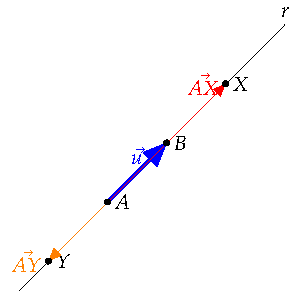
\includegraphics{equacao-vetorial-reta-plano-cartesiano.pdf}
  % \begin{tikzpicture}
  %   \coordinate[label=right:$A$] (A) at (0,0);
  %   \coordinate (U) at (-1.5,-1.5);
  %   \coordinate (V) at (3,3);
  %   \coordinate[label=right:$B$] (B) at (1,1);
  %   \coordinate[label=right:$X$] (X) at (2,2);
  %   \coordinate[label=right:$Y$] (Y) at (-1,-1);

  %   \draw (U) -- (V)
  %   node[at end,above]{$r$};

  %   \draw[ultra thick,->,>=triangle 45,blue] (A) -- (B)
  %   node[midway,above]{$\vec{u}$};
  %   \draw[->,>=triangle 45,red] (A) -- (X)
  %   node[at end,left,red]{$\vec{AX}$};
  %   \draw[->,>=triangle 45,orange] (A) -- (Y)
  %   node[at end,left,orange]{$\vec{AY}$};
  %   \foreach \p in {A,B,X,Y} \fill (\p) circle (0.5mm);
  %   \end{tikzpicture}  
\end{figure}

Ou seja, se e somente se, existe um n\'umero real $\lambda$ tal que
\begin{equation}\label{equacao_vetorial_reta_plano}
  \vec{AX} = \lambda\vec{u}.
\end{equation}

Assim para cada $\lambda \in \real$ fica definido um ponto $X$ na reta $r$ e se $X$ \'e um ponto da reta $r$, ent\~ao existe um n\'umero real $\lambda$ tal que $\vec{AX} = \lambda\vec{u}$.

\begin{definicao}\index{Reta no Plano!Equa\c{c}\~ao Vetorial}
  A equa\c{c}\~ao \eqref{equacao_vetorial_reta_plano} \'e chamada de \textbf{equa\c{c}\~ao vetorial da reta} $r$ ou \textbf{equa\c{c}\~ao da reta} $r$ \textbf{na forma vetorial}.
\end{definicao}

\begin{exemplos}
  Seja $r$ uma reta passando pelos pontos $A(1,2)$ e $B(-1, 3)$. Determine sua equa\c{c}\~ao vetorial.
  \begin{solucao}
    Um vetor diretor da reta $r$ pode ser tomado como sendo $\vec{u} = \vec{AB} = (-2, 1)$. Assim a equa\c{c}\~ao vetorial de $r$ ser\'a:
    \[
      \vec{AX} = \lambda\vec{u} = \lambda(-2,1), \quad \lambda \in \real.
    \]
    Podemos tamb\'em tomar como vetor diretor de $r$ o vetor $\vec{v} = \vec{BA} = (2,-1)$. Da{\'\i} a equa\c{c}\~ao vetorial de $r$ ser\'a
    \[
      \vec{AX} = \alpha\vec{v} = \alpha(2, -1), \quad \alpha \in \real.
    \]
  \end{solucao}
\end{exemplos}

\begin{observacao}
  Como o ponto e o vetor diretor de uma reta $r$ s\~ao escolhidos arbitrariamente, existem infinitas equa\c{c}\~oes vetorias para uma mesma reta $r$. Por exemplo, se $A$ e $B$ s\~ao pontos distintos de uma reta $r$, ent\~ao $\vec{AB}$ e $\vec{BA}$ s\~ao vetores diretores distintos de $r$ e portanto temos as equa\c{c}\~oes vetoriais
  \begin{align*}
    \vec{AX} = \lambda\vec{AB}\\
    \vec{AX} = \alpha\vec{BA}.
  \end{align*}
  Na verdade, qualquer vetor m\'ultiplo do vetor $\vec{AB}$ pode ser tomado como vetor diretor de $r$.
\end{observacao}

Agora, seja $\vec{u} = (a, b)$ um vetor diretor de uma reta $r$. Dado um ponto $A = (x_0, y_0)$ de $r$ o ponto $X = (x, y)$ pertence a reta $r$ se, e somente se, existe $\lambda \in \real$ tal que
\begin{align*}
  \vec{AX} &= \lambda\vec{u}\\
  (x - x_0, y - y_0) &= (\lambda a, \lambda b).
\end{align*}

Assim a reta $r$ pode ser descrita pelas equa\c{c}\~oes
\begin{equation}\label{equacao_parametrica_reta_plano}
  \begin{cases}
    x = x_0 + \lambda a\\
    x = y_0 + \lambda b 
  \end{cases}, \lambda \in \real
\end{equation}

\begin{definicao}\index{Reta no Plano!Equa\c{c}\~ao Param\'etrica}
  O sistema de equa\c{c}\~oes \eqref{equacao_parametrica_reta_plano} \'e chamado \textbf{sistema de equa\c{c}\~oes param\'etricas da reta} $r$ ou \textbf{sistema de equa\c{c}\~oes da reta} $r$ \textbf{na forma param\'etrica}.
\end{definicao}

\begin{exemplos}
  \begin{enumerate}
    \item O sistema de equa\c{c}\~oes
    \[
      \begin{cases}
        x = 1 + 2\lambda\\
        x = 2 - 3\lambda
      \end{cases}, \lambda \in \real
    \]
    define uma reta $r$ que passa pelo ponto $A(1,2)$ e que possui vetor diretor $\vec{u} = (2, -3)$.
    \item Seja $r$ a reta dada pelas equa\c{c}\~oes param\'etricas
    \[
      \begin{cases}
        x = 2 + 3t\\
        y = 1 + 4t
      \end{cases}, t\in \real.
    \]
    O ponto $(11, 13)$ pertence a $r$? E o ponto $(5,6)$?
    \begin{solucao}
      Para que o ponto $(11,13)$ perten\c{c}a a reta $r$ \'e preciso que exista $t \in \real$ tal que
      \begin{align*}
        11 = 2 + 3t\\
        13 = 1 + 4t.
      \end{align*}
    Cuja solu\c{c}\~ao \'e $t = 3$. Logo o ponto $(11,13)$ pertence a reta $r$.

    Para que o ponto $(5,6)$ perten\c{c}a a reta $r$ \'e preciso que exista $t \in \real$ tal que
      \begin{align*}
        5 = 2 + 3t\\
        6 = 1 + 4t.
      \end{align*}
    Resolvendo, obtemos $t = 1$ e $t = 5/4$. Logo o ponto $(5,6)$ n\~ao pertence a reta $r$.
    \end{solucao}
  \end{enumerate}
\end{exemplos}

Seja $r$ uma reta com vetor diretor $\vec{u} = (a,b)$, onde $ab\ne 0$ e que passa pelo ponto $(x_0, y_0)$. Sabemos que sua equa\c{c}\~ao param\'etrica \'e
\[
  \begin{cases}
    x = x_0 + \lambda a\\
    y = y_0 + \lambda b.
  \end{cases}
\]
Isolando $\lambda$ nas duas equa\c{c}\~oes encontramos
\[
  \lambda = \dfrac{x - x_0}{a}\quad \lambda = \dfrac{y - y_0}{b},
\]
isto \'e, a equa\c{c}\~ao
\begin{equation}\label{equacao_simetrica_reta_plano}
  \dfrac{x - x_0}{a} = \dfrac{y - y_0}{b}.
\end{equation}
determina se um ponto pertence a reta $r$ ou n\~ao.

\begin{definicao}\index{Reta no Plano!Equa\c{c}\~ao Sim\'etrica}
  A equa\c{c}\~ao \eqref{equacao_simetrica_reta_plano} \'e chamada de \textbf{sistema de equa\c{c}\~oes da reta} $r$ \textbf{na forma sim\'etrica} ou por abuso de linguagem, \textbf{equa\c{c}\~oes da reta} $r$ \textbf{na forma sim\'etrica}.
\end{definicao}

\begin{exemplos}
 Encontre a equa\c{c}\~ao sim\'etrica da reta $r$ que passa pelos pontos $A(-1,2)$ e $B(3,4)$. O ponto $(0,5/2)$ est\'a na reta $r$? E o ponto $(1,2)$?
 \begin{solucao}
   Um vetor diretor para a reta $r$ \'e dado por $\vec{u} = \vec{AB} = (4,2)$. Assim usando o ponto $A$ a equa\c{c}\~ao sim\'etrica de $r$ \'e
   \[
     \dfrac{x + 1}{4} = \dfrac{y - 2}{2}.
   \]
 Como
 \[
    \dfrac{0 + 1}{4} = \dfrac{\dfrac{5}{2} - 2}{2}
 \]
 ent\~ao o ponto $(0,5/2)$ est\'a na reta $r$. Agora como
 \[
  \dfrac{1+1}{4} \ne \dfrac{2 - 2}{2}
 \]
 o ponto $(1, 2)$ n\~ao est\'a na reta $r$.

 \end{solucao}
\end{exemplos}

\begin{observacao}
  \begin{enumerate}
    \item Para que uma equa\c{c}\~ao de uma reta $r$ esteja na forma \eqref{equacao_parametrica_reta_plano} \'e obrigat\'orio que o coeficente de $x$ e $y$ sejam 1. Assim, por exemplo a equa\c{c}\~ao na forma
    \[
      \begin{cases}
        2x = 1 - 3\lambda\\
        -y = 2 + \lambda
      \end{cases}
    \]
    n\~ao ser\'a considerada como uma equa\c{c}\~ao param\'etica de uma reta. Do mesmo modo, uma equa\c{c}\~ao do tipo
    \[
      \dfrac{2x - 7}{3} = \dfrac{y}{2}
    \]
    n\~ao ser\'a considerada uma equa\c{c}\~ao sim\'etrica de uma reta $r$ pois n\~ao est\'a na forma \eqref{equacao_simetrica_reta_plano}.

    \item Cada tipo de equa\c{c}\~ao da reta apresenta sua vantagens. A forma vetorial descreve uma reta tanto no plano cartesiano como no espa\c{c}o tridimensional e mesmo em espa\c{c}os ``maiores''. A forma param\'etrica reduz o n\'umero de inc\'ognitas com as quais precisamos trabalhar. Neste tipo de equa\c{c}\~ao lidamos com somente uma inc\'ognita em vez de duas. J\'a a forma sim\'etrica exibe qual a rela\c{c}\~ao que as coordenadas dos pontos de uma reta devem satisfazer entre si.
  \end{enumerate}
\end{observacao}

Seja $r$ uma reta que cont\'em o ponto $(x_0, y_0)$ e com vetor diretor $\vec{u} = (a, b)$. Sua equa\c{c}\~ao param\'etrica \'e
  \begin{numcases}{}
    x = x_0 + \lambda a\label{eq_parametrica1}\\
    y = y_0 + \lambda b.\label{eq_parametrica2}
  \end{numcases}

Multiplicando a equa\c{c}\~ao \eqref{eq_parametrica1} por $b$ e a equa\c{c}\~ao \eqref{eq_parametrica2} por $a$ obtemos
\begin{align}
  bx = bx_0 + \lambda ab\label{eq_parametrica_auxiliar1}\\
  ay = ay_0 + \lambda ab.\label{eq_parametrica_auxiliar2}
\end{align}

Fazendo \eqref{eq_parametrica_auxiliar2} - \eqref{eq_parametrica_auxiliar1} obtemos
\[
  ay - bx = ay_0 - bx_0.
\]

Agora note que $ay_0 - bx_0$ \'e uma constante. Assim fazendo, $c = ay_0 - bx_0$ podemos escrever
\begin{equation}\label{equacao_cartesiana_reta_plano}
  ay - bx = c
\end{equation}
que \'e chamada de \textbf{equa\c{c}\~ao cartesiana da reta} $r$.\index{Reta no Plano!Equa\c{c}\~ao Cartesiana}

Observe que ser o vetor diretor $\vec{u} = (a,b)$ da reta $r$  \'e tal que $a = 0$, obtemos a equa\c{c}\~ao $x = x_0$ e a reta $r$ \'e paralela ao eixo $y$. Caso $b = 0$, obtemos $y = y_0$ e a reta \'e paralela ao eixo $x$.
\begin{figure}[!h]
  \centering
  \caption{Retas paralelas aos eixos}
  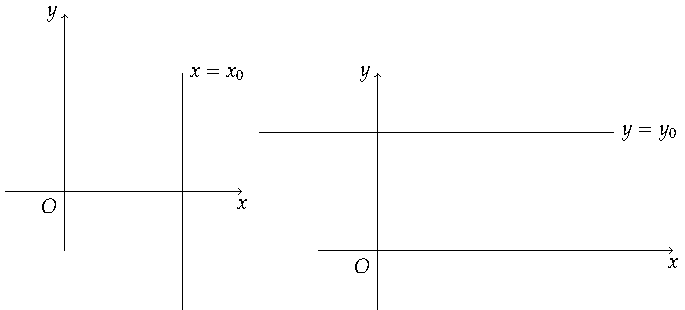
\includegraphics{retas-paralelas-plano-cartesiano.pdf}
  % \begin{tikzpicture}[scale=2]
  %   \coordinate[label=below left:$O$] (A) at (-3,0);
  %   \coordinate (W) at (-2,-1);
  %   \coordinate (V) at (-2,1);
  %   %defini\c{c}\~ao das coordenadas dos eixos cartesianos
  %   \coordinate (F) at (-3.5,0);
  %   \coordinate (G) at (-3,-0.5);
  %   \coordinate (X) at (-1.5,0);
  %   \coordinate (Y) at (-3,1.5);
  %   % Styles
  %   \tikzstyle{axes}=[]

  %   \begin{scope}[style=axes]%constr\'oi os eixos cartesianos
  %     \draw[->] (F) -- (X) node[below] {$x$} coordinate(x axis);
  %     \draw[->] (G) -- (Y) node[left] {$y$} coordinate(y axis);
  %   \end{scope}

  %   \draw  (V) -- (W)
  %     node[at start, right]{$x = x_0$};
  %   \end{tikzpicture}
  %   \begin{tikzpicture}[scale=2]
  %   \coordinate[label=below left:$O$] (A) at (0,0);
  %   \coordinate (W) at (-1,1);
  %   \coordinate (V) at (2,1);
  %   %defini\c{c}\~ao das coordenadas dos eixos cartesianos
  %   \coordinate (F) at (-0.5,0);
  %   \coordinate (G) at (0,-0.5);
  %   \coordinate (X) at (2.5,0);
  %   \coordinate (Y) at (0,1.5);
  %   % Styles
  %   \tikzstyle{axes}=[]

  %   \begin{scope}[style=axes]%constr\'oi os eixos cartesianos
  %     \draw[->] (F) -- (X) node[below] {$x$} coordinate(x axis);
  %     \draw[->] (G) -- (Y) node[left] {$y$} coordinate(y axis);
  %   \end{scope}

  %   \draw  (V) -- (W)
  %     node[at start, right]{$y = y_0$};
  %   \end{tikzpicture}
\end{figure}

Se $a \ne 0$, ent\~ao podemos dividir a equa\c{c}\~ao \eqref{equacao_cartesiana_reta_plano} por $a$ obtendo
\[
  y = \dfrac{b}{a}x + \dfrac{c}{a}.
\]
Fazendo $m = b/a$ e $k = c/a$ temos a equa\c{c}\~ao
\[
  y = mx + k,
\]
onde $m = b/a = \tan \theta$.

Note que o vetor $\vec{v} = (1,m)$ \'e paralelo \`a reta $r$ de equa\c{c}\~ao $y = mx + k$. De fato,
\begin{align*}
  \vec{v} = (1,m) = \left(1, \dfrac{b}{a}\right) = \dfrac{1}{a}(a,b) = \dfrac{1}{a}\vec{u}.
\end{align*}

\begin{exemplos}
  Determine as equa\c{c}\~oes param\'etricas e cartesianas da reta $r$ definida pelos pontos $A(1,5)$ e $B(2,7)$.
  \begin{solucao}
    Um vetor diretor de $r$ \'e dado por $\vec{u} = \vec{AB} = (1,2)$. Assim $m = b/a$ onde $\vec{u} = (a,b)$ vale $m = 2$. Desse modo temos
    \[
      y = 2x + k.
    \]
    Como o ponto $A = (1,5)$ pertence a reta $r$ devemos ter
    \[
      5 = 2(1) + k
    \]
    donde $k = 3$. Portanto a equa\c{c}\~ao cartesiana de $r$ ser\'a
    \[
      y = 2x + 3.
    \]
    A equa\c{c}\~ao param\'etrica ser\'a
    \[
      \begin{cases}
        x = 1 + \lambda\\
        y = 5 + 2\lambda
      \end{cases}, \lambda \in \real
    \]
    caso escolhamos o ponto $A$. As equa\c{c}\~oes param\'etricas de $r$ tamb\'em podem ser expressas como
    \[
      \begin{cases}
        x = 2 + \lambda\\
        y = 7 + 2\lambda
      \end{cases}, \lambda \in \real
    \]
    caso escolhamos o ponto $B$.
  \end{solucao}
\end{exemplos}
% section equacoes_da_reta (end)

\section{\^Angulo entre retas} % (fold)
\label{sec:angulo_entre_retas}
Sejam $r$ uma reta passando pelo ponto $A(x_1, y_1)$ e com vetor diretor $\vec{u} = (a,b)$ e $s$ uma reta passando pelo ponto $B(x_2, y_2)$ e com vetor diretor $\vec{v} = (c,d)$. O \textbf{\^angulo entre duas retas} $r$ e $s$ \'e definido como o menor \^angulo entre o vetor diretor $\vec{u}$ de $r$ e o vetor diretor $\vec{v}$ de $s$.

\begin{figure}[!h]
  \centering
  \caption{\^Angulo entre retas}
  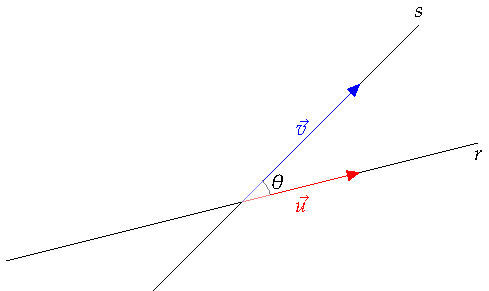
\includegraphics{angulo-retas-plano-cartesiano.pdf}
  % \begin{tikzpicture}
  %   \coordinate (A) at (0,0);
  %   \coordinate (B) at (-4,-1);
  %   \coordinate (X) at (4,1);
  %   \coordinate (C) at (-1.5,-1.5);
  %   \coordinate (Y) at (3,3);
  %   \coordinate (U) at (2,0.5);
  %   \coordinate (V) at (2,2);

  %   \draw (B) -- (X)
  %   node[at end,below]{$r$};
  %   \draw (C) -- (Y)
  %   node[at end,above]{$s$};

  %   \draw[->,>=triangle 45,red] (A) -- (U)
  %   node[midway,below]{$\vec{u}$};
  %   \draw[->,>=triangle 45,blue] (A) -- (V)
  %   node[midway,above]{$\vec{v}$};

  %   % Mark the angle XAY
  %   \begin{scope}
  %     \path[clip] (A) -- (X) -- (Y);
  %     \fill[white, opacity=0.5, draw=black] (A) circle (5mm);
  %     \node at ($(A)+(30:7mm)$) {$\theta$};
  %   \end{scope}
  % \end{tikzpicture}
\end{figure}

Assim o \^angulo $\theta$ entre $r$ e $s$ \'e dado por
\[
  \cos\theta = \dfrac{\mid\inner{u}{v}\mid}{\norm{\vec{u}}\norm{\vec{v}}},\quad 0 \le \theta \le \dfrac{\pi}{2}
\]

\begin{exemplos}
  Determine o \^angulo entre as retas $r$ e $s$ cujas equa\c{c}\~oes s\~ao:
  \begin{align*}
    r: y = 2x -2\\
    s: y = -x + 4.
  \end{align*}
  \begin{solucao}
    Temos $m = b/a$, onde $a$ e $b$ s\~ao as coordenadas do vetor diretor da reta em quest\~ao. Assim pondemos tomar $\vec{u} = (1,2)$ como um vetor diretor de $r$ e $\vec{v} = (-1,1)$ como um vetor diretor de $s$. Da{\'\i}
    \[
      \cos\theta = \dfrac{\mid\inner{u}{v}\mid}{\norm{\vec{u}}\norm{\vec{v}}} = \dfrac{1}{\sqrt{10}}.
    \]
    Logo $\theta = \arccos\left(\dfrac{\sqrt{10}}{10}\right)$.
  \end{solucao}
\end{exemplos}
% section angulo_entre_retas (end)

\section{Dist\^ancia de um ponto a uma reta} % (fold)
\label{sec:distancia_de_um_ponto_a_uma_reta}
A dist\^ancia de um ponto $P(x_0,y_0)$ \`a reta $r$ de equa\c{c}\~ao $y = mx + k$ \'e definida como sendo a dist\^ancia de $P$ ao ponto $A(x_1, y_1)$, onde $A$ \'e o p\'e da perpendicular \`a reta $r$ passando pelo ponto $P$.
\begin{figure}[!h]
  \centering
  \caption{Dist\^ancia de ponto a reta}
  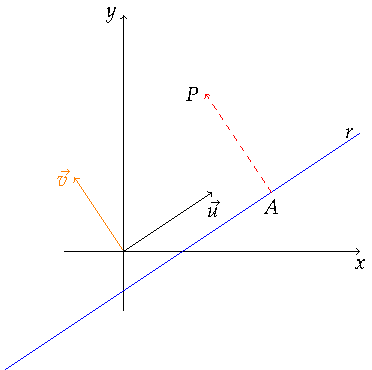
\includegraphics{distancia-ponto-reta-plano-cartesiano.pdf}
  % \begin{tikzpicture}[scale=2]%soma de vetores no plano
  %   \coordinate (D) at (-1,-1);
  %   \coordinate[label=left:$r$] (B) at (2,1);
  %   \coordinate (U) at ($0.25*(B)-0.25*(D)$);
  %   \coordinate (V) at ($(0,0)!0.75cm!90:(U)$);
  %   \draw[->,color=black] (0,0) -- (U)
  %     node[at end, below]{$\vec{u}$};
  %   \draw[->,orange] (0,0) -- (V)
  %     node[at end, left]{$\vec{v}$};
  %   \coordinate[label=below:$A$] (A) at ($(D)!.75!(B)$);
  %   \coordinate[label=left:$P$] (P) at ($(A)!1cm!90:(B)$);
  %   %defini\c{c}\~ao das coordenadas dos eixos cartesianos
  %   \coordinate (F) at (-0.5,0);
  %   \coordinate (G) at (0,-0.5);
  %   \coordinate (X) at (2,0);
  %   \coordinate (Y) at (0,2);
  %   % Styles
  %   \tikzstyle{axes}=[]

  %   \begin{scope}[style=axes]%constr\'oi os eixos cartesianos
  %     \draw[->] (F) -- (X) node[below] {$x$} coordinate(x axis);
  %     \draw[->] (G) -- (Y) node[left] {$y$} coordinate(y axis);
  %   \end{scope}

  %   \draw[blue] (D)--(B);
  %   \draw[->,red,dashed] (A) -- (P);
  % \end{tikzpicture}
\end{figure}
Agora note que o vetor $\vec{u} = (1,m)$ \'e paralelo \`a reta $r$. Al\'em disso, o vetor $\vec{v} = (-m, 1)$ \'e tal que $\vec{u}\cdot\vec{v} = 0$, isto \'e, $\vec{u}\perp\vec{v}$. Portanto, $\vec{AP}\varparallel\vec{v}$ e ent\~ao existe $\lambda \in \real$ tal que
\[
  \vec{AP} = \lambda\vec{v}.
\]
Logo
\begin{equation}\label{distancia_ponto_reta_plano}
  d(P,r) = \norm{\vec{AP}} = \norm{\lambda\vec{v}} = \mid\lambda\mid \norm{\vec{v}} = \mid\lambda\mid\sqrt{m^2 + 1}.
\end{equation}
Assim para determinarmos $d(P,r)$ basta conhecer $\lambda$. Agora,
\[
  \vec{PA} = (x_1 - x_0, y_1 - y_0) = \lambda(-m, 1)
\]
donde
\begin{align*}
  x_1 = x_0 - \lambda m\\
  y_1 = y_0 + \lambda.
\end{align*}
Como $A(x_1, y_1)$ pertence a reta $r$, devemos ter
\begin{align*}
  y_1 = mx_1 + k\\
  y_0 + \lambda = m(x_0 - \lambda m) + k\\
  y_0 + \lambda = mx_0 - \lambda m^2 + k\\
  \lambda = \dfrac{-y_0 + mx_0 + k}{1 + m^2}.
\end{align*}
Substituindo $\lambda$ em \eqref{distancia_ponto_reta_plano}
\[
  d(P, r) = \left|\dfrac{-y_0 + mx_0 + k}{1 + m^2}\right|\sqrt{m^2 + 1}.
\]
Portanto
\[
  d(P, r) = \dfrac{\mid mx_0 + k - y_0\mid}{\sqrt{m^2 + 1}}
\]
\'e a express\~ao para a dist\^ancia de um ponto $P(x_0,y_0)$ at\'e uma reta $r$ de equa\c{c}\~ao $y = mx + k$.

\begin{exemplos}
  Seja $r$ a reta de equa\c{c}\~ao $y = 3x - 1$. Qual a dist\^ancia do ponto $P(2,2)$ \`a reta $r$?
  \begin{solucao}
    \[
      d(P,r) = \dfrac{\mid 3(2) - 1 - 2\mid}{\sqrt{3^2 + 1}} = \dfrac{3}{\sqrt{10}}.
    \]
  \end{solucao}
\end{exemplos}
% section distancia_de_um_ponto_a_uma_reta (end)



% chapter reta_no_plano (end)